% !TEX root = ../discretemath.tex

\section{Дискретное математическое ожидание и примеры распределений}

\subsection{Случайная величина}

\begin{Definition}{Случайная величина}{}
	Пусть $\Omega$ — вероятностное пространство. Функция $\xi \colon \Omega \to \mathbb{R}$ называется \textbf{случайной величиной} (с.в.).
\end{Definition}

Пространство $\Omega$ разбивается на слои по значениям с.в.:
\[
\Omega = \bigsqcup_{x \in \mathbb{R}} A_x, \qquad A_x = \{\omega \in \Omega : \xi(\omega) = x\},
\qquad
\Pr[\xi = x] := \Pr[A_x].
\]

\begin{Example}{Минимум при трёх бросках кубика}{}
	$\xi$ — минимальное из трёх выпавших чисел. Тогда
	\[
	\Pr[\xi = 3] = \Pr[\xi \ge 3] - \Pr[\xi \ge 4]
	= \left(\tfrac{4}{6}\right)^3 - \left(\tfrac{3}{6}\right)^3
	= \frac{64 - 27}{216} = \frac{37}{216}.
	\]
\end{Example}

\begin{Example}{Количество единиц при трёх бросках}{}
	$\beta$ — число выпавших единиц. Тогда
	\[
	\Pr[\beta = 2] = \binom{3}{2}\left(\tfrac{1}{6}\right)^2\tfrac{5}{6} = \frac{5}{72}.
	\]
\end{Example}

\begin{Example}{Индикаторная случайная величина}{}
	Для $A\subseteq\Omega$ \textbf{индикатор} — это с.в. $\delta\colon\Omega\to\{0,1\}$:
	\[
	\delta(\omega)=\begin{cases}0,&\omega\notin A,\\ 1,&\omega\in A.\end{cases}
	\]
	Индикаторы — главный инструмент при подсчёте матожидания «числа событий».
\end{Example}

\subsection{Независимость случайных величин}

\begin{Definition}{Независимость двух с.в.}{}
	С.в. $\xi$ и $\beta$ \textbf{независимы}, если для любых $a,b\in\mathbb{R}$ события $[\xi=a]$ и $[\beta=b]$ независимы:
	\[
	\Pr[\xi=a,\ \beta=b]=\Pr[\xi=a]\cdot\Pr[\beta=b].
	\]
\end{Definition}

\begin{Definition}{Независимость в совокупности}{}
	С.в. $\xi_1,\dots,\xi_n$ \textbf{независимы в совокупности}, если для любых $a_1,\dots,a_n\in\mathbb{R}$
	\[
	\Pr[\xi_1=a_1,\ \dots,\ \xi_n=a_n]=\prod_{i=1}^n\Pr[\xi_i=a_i].
	\]
\end{Definition}

\begin{Statement}{}{}
	Если события $A,B\subseteq\Omega$ независимы, то их индикаторы $\chi_A,\chi_B$ — независимые с.в.
\end{Statement}

\subsection{Плотность и функция распределения}

\begin{Definition}{Плотность (функция вероятностей)}{}
	\textbf{Плотность} с.в. $\xi$ — функция $d_\xi\colon\mathbb{R}\to[0,1]$, $d_\xi(x)=\Pr[\xi=x]$.
\end{Definition}

\begin{Definition}{Функция распределения}{}
	\textbf{Функция распределения} с.в. $\xi$ — функция $F_\xi\colon\mathbb{R}\to[0,1]$:
	\[
	F_\xi(x)=\sum_{y\le x}\Pr[\xi=y]=\Pr[\xi\le x].
	\]
\end{Definition}

\begin{Remark}{}{}
	$F_\xi$ неубывающая, непрерывная справа, со скачками величины $\Pr[\xi=x]$ в точках $x$, и $F_\xi(-\infty)=0$, $F_\xi(+\infty)=1$.
\end{Remark}

\subsection{Примеры распределений}

\subsubsection*{Распределение Бернулли}

\begin{Example}{Распределение Бернулли}{}
	Значение $0$ с вероятностью $p$, значение $1$ — с вероятностью $1-p$. Плотность $d(0)=p$, $d(1)=1-p$; функция распределения
	\[
	F(x)=\begin{cases}0,&x<0,\\ p,&0\le x<1,\\ 1,&1\le x.\end{cases}
	\]
\end{Example}

\begin{figure}[H]
	\centering
	\begin{tikzpicture}[font=\small, >=Stealth, scale=1.0]
		\draw[->] (-1.2,0) -- (3.2,0) node[right]{$x$};
		\draw[->] (0,-0.2) -- (0,2.2) node[above]{$F(x)$};
		\draw[dashed] (-1.2,0.8) -- (3.0,0.8) node[right]{};
		\draw[dashed] (-1.2,1.6) -- (3.0,1.6);
		\node[left] at (0,0.8) {$p$};
		\node[left] at (0,1.6) {$1$};
		% ступени: F=0 при x<0, F=p при 0<=x<1, F=1 при x>=1
		\draw[very thick, blue] (-1.2,0) -- (0,0);
		\draw[very thick, blue] (0,0.8) -- (1,0.8);
		\draw[very thick, blue] (1,1.6) -- (3.0,1.6);
		% открытые/закрытые точки
		\filldraw[blue] (0,0.8) circle (1.6pt); \draw[blue] (0,0) circle (1.6pt);
		\filldraw[blue] (1,1.6) circle (1.6pt); \draw[blue] (1,0.8) circle (1.6pt);
		\node[below] at (0,-0.05) {$0$}; \node[below] at (1,-0.05) {$1$};
	\end{tikzpicture}
	\caption{Функция распределения Бернулли: ступенчатая, со скачками $p$ в точке $0$ и $1-p$ в точке $1$. Высота каждого скачка равна вероятности соответствующего значения.}
\end{figure}

\subsubsection*{Биномиальное распределение}

\begin{Example}{Биномиальное распределение $\mathrm{Bin}(n,p)$}{}
	$n$ независимых испытаний, в каждом «успех» с вероятностью $p$; $\xi$ — число успехов. Тогда
	\[
	d(k)=\binom{n}{k}p^k(1-p)^{n-k},\qquad k=0,1,\dots,n.
	\]
\end{Example}

\begin{figure}[H]
	\centering
	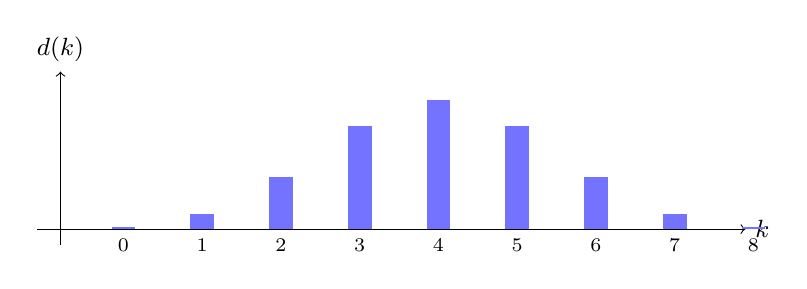
\begin{tikzpicture}[font=\small, scale=1.0]
		\draw[->] (-0.3,0) -- (8.7,0) node[right]{$k$};
		\draw[->] (0,-0.2) -- (0,2.0) node[above]{$d(k)$};
		% Bin(8, 0.5): высоты пропорциональны C(8,k)/256, масштаб x6
		\foreach \k/\h in {0/0.02,1/0.19,2/0.66,3/1.31,4/1.64,5/1.31,6/0.66,7/0.19,8/0.02}{
			\fill[blue!55] (\k+0.65,0) rectangle (\k+0.95,\h);
			\node[below] at (\k+0.8,0) {\scriptsize\k};
		}
	\end{tikzpicture}
	\caption{Плотность $\mathrm{Bin}(8,\tfrac12)$: «колоколообразная», симметричная относительно среднего $np=4$. У биномиального распределения $\mathbb{E}[\xi]=np$.}
\end{figure}

\subsection{Математическое ожидание}

\begin{Definition}{Математическое ожидание}{}
	\textbf{Математическое ожидание} с.в. $\xi$:
	\[
	\mathbb{E}[\xi]:=\sum_{x\in\mathbb{R}}\Pr[\xi=x]\cdot x=\sum_{\omega\in\Omega}\Pr[\omega]\cdot\xi(\omega).
	\]
\end{Definition}

\begin{Statement}{}{}
	Для константы $c\in\mathbb{R}$: $\ \mathbb{E}[c\cdot\xi]=c\cdot\mathbb{E}[\xi]$.
\end{Statement}

\begin{Statement}{Линейность математического ожидания}{}
	Для любых с.в. $\xi_1,\dots,\xi_n$:
	\[
	\mathbb{E}[\xi_1+\cdots+\xi_n]=\mathbb{E}[\xi_1]+\cdots+\mathbb{E}[\xi_n].
	\]
\end{Statement}

\begin{Remark}{}{}
	Линейность верна \emph{без всякого предположения о независимости} — это её главная сила. Например, матожидание числа неподвижных точек случайной перестановки $=\sum_i\Pr[\sigma(i)=i]=n\cdot\tfrac1n=1$.
\end{Remark}

\begin{Theorem}{Формула полного математического ожидания}{}
	Пусть $\Omega=A_1\sqcup\cdots\sqcup A_n$ — разбиение. Тогда
	\[
	\mathbb{E}[\xi]=\sum_i\mathbb{E}[\xi\mid A_i]\cdot\Pr[A_i].
	\]
\end{Theorem}

\begin{proof}
	\begin{align*}
		\mathbb{E}[\xi]
		&=\sum_x x\cdot\Pr[\xi=x]
		=\sum_x x\cdot\sum_{i=1}^n\Pr[\xi=x\mid A_i]\Pr[A_i]\\
		&=\sum_{i=1}^n\Bigl(\sum_x \Pr[\xi=x\mid A_i]\cdot x\Bigr)\Pr[A_i]
		=\sum_{i=1}^n\mathbb{E}[\xi\mid A_i]\Pr[A_i].
	\end{align*}
\end{proof}

\subsection{Геометрическое распределение}

Монета даёт $1$ с вероятностью $p$ и $0$ с вероятностью $1-p$; бросаем до первого $1$.

\begin{Example}{Геометрическое распределение}{}
	$\xi$ — номер первого успеха. При $p>0$:
	\[
	\Pr[\xi=k]=(1-p)^{k-1}p,\qquad k=1,2,3,\dots
	\]
	Нормировка: $\sum_{k\ge 1}(1-p)^{k-1}p=1$.
\end{Example}

Вычислим $\mathbb{E}[\xi]$ через формулу полного матожидания (по первому броску):
\begin{align*}
	\mathbb{E}[\xi]
	&=\sum_{k\ge 1}k(1-p)^{k-1}p
	=p\bigl(1+(1-p)+(1-p)^2+\cdots\bigr)+\sum_{k\ge 2}(k-1)(1-p)^{k-1}p\\
	&=1+(1-p)\sum_{k\ge 2}(k-1)(1-p)^{k-2}p
	=1+(1-p)\,\mathbb{E}[\xi].
\end{align*}
Из уравнения $\mathbb{E}[\xi]=1+(1-p)\mathbb{E}[\xi]$ получаем
\[
\mathbb{E}[\xi]=\frac1p.
\]

\subsection{Распределение Пуассона}

\begin{Definition}{Распределение Пуассона}{}
	С.в. $\xi$ имеет \textbf{распределение Пуассона} с параметром $\lambda>0$, если
	\[
	\Pr[\xi=k]=\frac{\lambda^k}{k!}\,e^{-\lambda},\qquad k=0,1,2,\dots
	\]
\end{Definition}

\subsubsection*{Связь с биномиальным распределением}

Возьмём $\mathrm{Bin}(n,p)$ с $p=\tfrac{\lambda}{n}$ и устремим $n\to\infty$:
\[
\Pr[\xi=k]=\binom{n}{k}p^k(1-p)^{n-k}
=\underbrace{\frac{n(n-1)\cdots(n-k+1)}{n^k}}_{\to 1}\cdot\frac{\lambda^k}{k!}\cdot\underbrace{\left(1-\tfrac{\lambda}{n}\right)^n}_{\to e^{-\lambda}}\cdot\underbrace{\frac{1}{\left(1-\tfrac{\lambda}{n}\right)^k}}_{\to 1}.
\]
В пределе получаем $\dfrac{\lambda^k}{k!}e^{-\lambda}$ — распределение Пуассона.

\subsubsection*{Математическое ожидание}

\begin{Statement}{}{}
	Если $\xi\sim\mathrm{Pois}(\lambda)$, то $\mathbb{E}[\xi]=\lambda$.
\end{Statement}

\begin{proof}
	\begin{align*}
		\mathbb{E}[\xi]
		&=\sum_{k\ge 0}k\cdot\frac{\lambda^k}{k!}e^{-\lambda}
		=\sum_{k\ge 1}\frac{\lambda^k}{(k-1)!}e^{-\lambda}
		=\lambda\sum_{i\ge 0}\frac{\lambda^i}{i!}e^{-\lambda}
		=\lambda.
	\end{align*}
\end{proof}
